\chapter{FFDA}
Log-based FFDA di sistemi complessi a larga scala. I dati sono stati collezionati dai supercalcolatori Mercury e Blue-Gene. 
\\Breve descrizione dell'architettura dei due sistemi
\section{Analisi dei log}
Formato entries per entrambi.
\\RICORDA!! I dati sono stati già filtrati, ma comunque sono presenti ridondanze. Quindi necessitano una manipolazione.
\section{Manipolazione}
Fatta tramite tecniche di coalescenza, le quali consentono di raggruppare entries ricercando correlazioni sui dati. 
\\Coalescenza spaziale: raggruppiamo entries provenienti da + nodi diversi cercando di capire se si sono verificate nello stesso intervallo temporale specificato dalla finestra temporale W seleizonata.
\subsection{Scelta W}
Si prova per vari valori di W, contando per ogni valore quante tuple vengono generate -> grafico -> prendiamo la W associata al suo knee.
\\
Generico:
\\
\\Mercury: DimWindow = 150
\\BlueGene: DimWindow = 150
\subsection{Analisi Truncation}
Per qualche tupla d'esempio individuare se sono presenti troncamenti.
\subsection{Analisi Collisions}
Per qualche tupla d'esempio individuare collissioni.
\subsection{Domanda 1}
La stessa finestra di coalescenza può essere usata per diversi nodi (fare sia per Mercury che BG) e categorie d'errore (solo Mercury)?
\section{Reliability Modeling}
Una volta ottenuti i dati manipolati è necessario procedere ad una loro analisi. In particolare, si parte dagli \textit{interarrivi} (file interarrivals.txt, ottenuto alla creazione delle tuple), i quali rappresentano la "distanza temporale" tra due tuple consecutive, ovvero il TTF - Time To Failure del sistema complessivo. 
\\L'obiettivo è valutare le distribuzioni empiriche di:
\begin{itemize}
	\item \textit{Tempi di Fallimento - Unreliability},
	\item \textit{Reliability}
\end{itemize}
Con il seguente script MATLAB è stata calcolata la CDF del TTF, e a partire da essa la Reliability empirica del sistema:
\begin{minted}[framesep = 1mm,
	fontsize = \footnotesize,
	breaklines,
	]{MATLAB}
	load interarrivals.txt;         
	[y,t] = cdfcalc(interarrivals); %ne calcolo la CDF = unreliability
	empTTF = y(2:size(y,1));        %scarto la prima riga (?)
	empRel = 1 - empTTF;            %Reliability
	plot(t,empTTF,'-*b');
	hold on;
	plot(t,empRel,'-+r');
	xlabel('time[s]');
	ylabel('p');
	legend('empTTF','empRel');
\end{minted}
\subsubsection{EmpTTF e EmpRel - Mercury}
\begin{figure}[H]
	\centering
	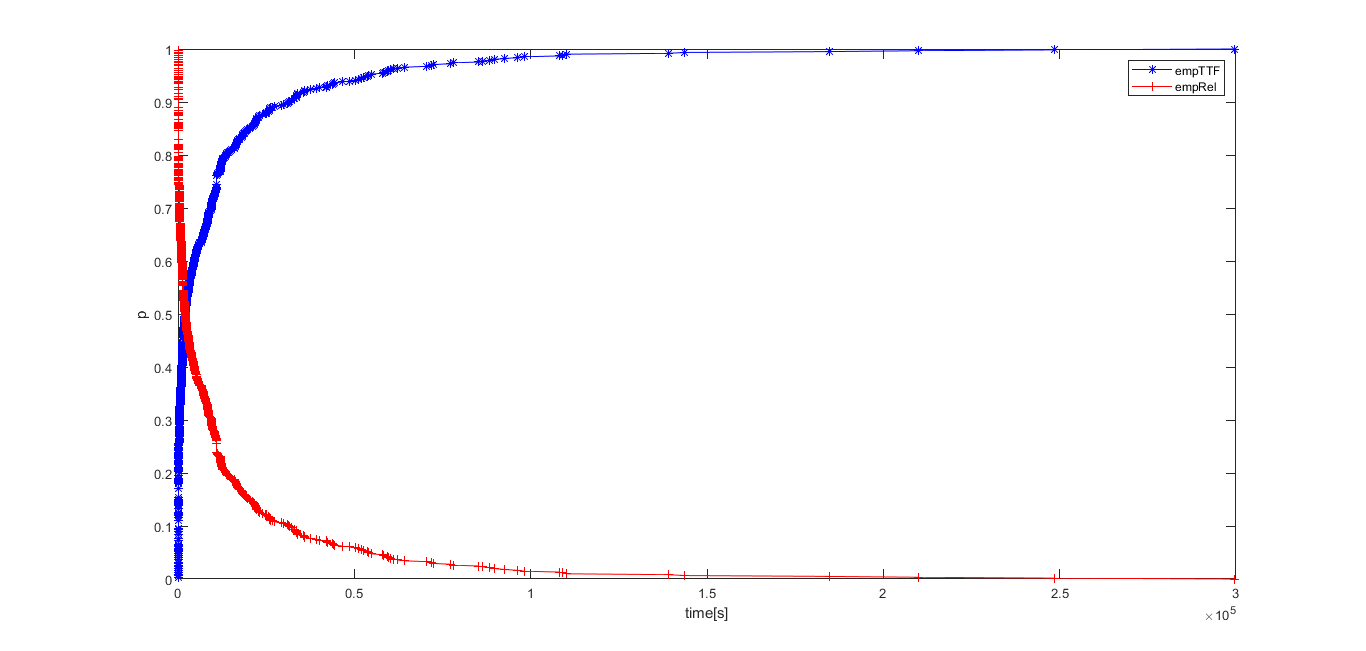
\includegraphics[width=\textwidth]{img/hw6/TTF_Mercury.png}
	\caption{\textit{Distribuzioni Empiriche Mercury}}
\end{figure}
\subsubsection{EmpTTF e EmpRel - BlueGene}
\begin{figure}[H]
	\centering
	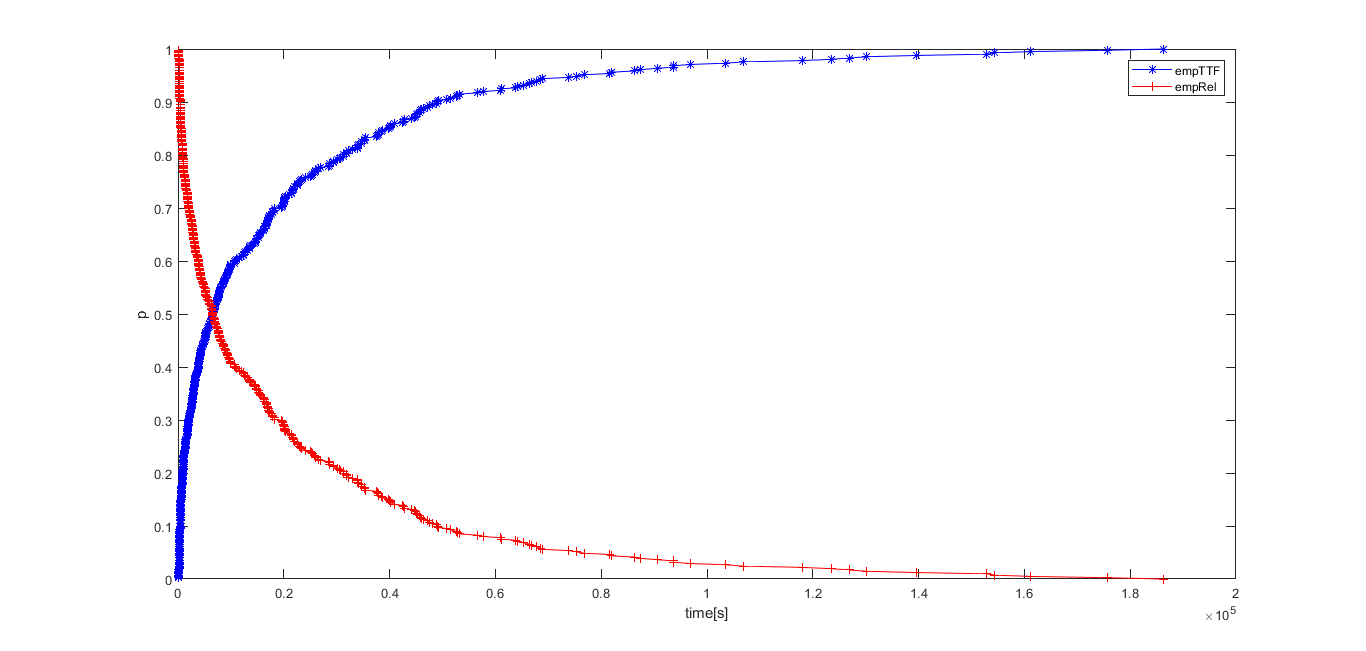
\includegraphics[width=\textwidth]{img/hw6/TTF_BG.png}
	\caption{\textit{Distribuzioni Empiriche Blue-Gene}}
\end{figure}
\subsection{Fitting di EmpRel}
Di tali distribuzioni opportunamente ottenute, bisogna effettuarne un \textit{Curve Fitting} in modo da ricavarne un modello statistico (così facendo ho informazioni anche sul probabile andamento futuro della curva). Tale operazione risulta essere fondamentale, in quanto una data distribuzione può essere sintomatica di un particolare guasto.
\\A tale scopo è stato utilizzato il tool MATLAB \textit{Curve Fitting}.
\subsubsection{Fitting EmpRel - Mercury}
Il fitting è stato eseguito con una distribuzione Esponenziale a 2 termini, descritta dalla seguente equazione:
\begin{equation*}
	f(x) = a*e^{bx}+c*e^{dx}
\end{equation*}
i cui coefficienti sono stati determinati tramite algoritmi interni del tool.
\begin{figure}[H]
	\centering
	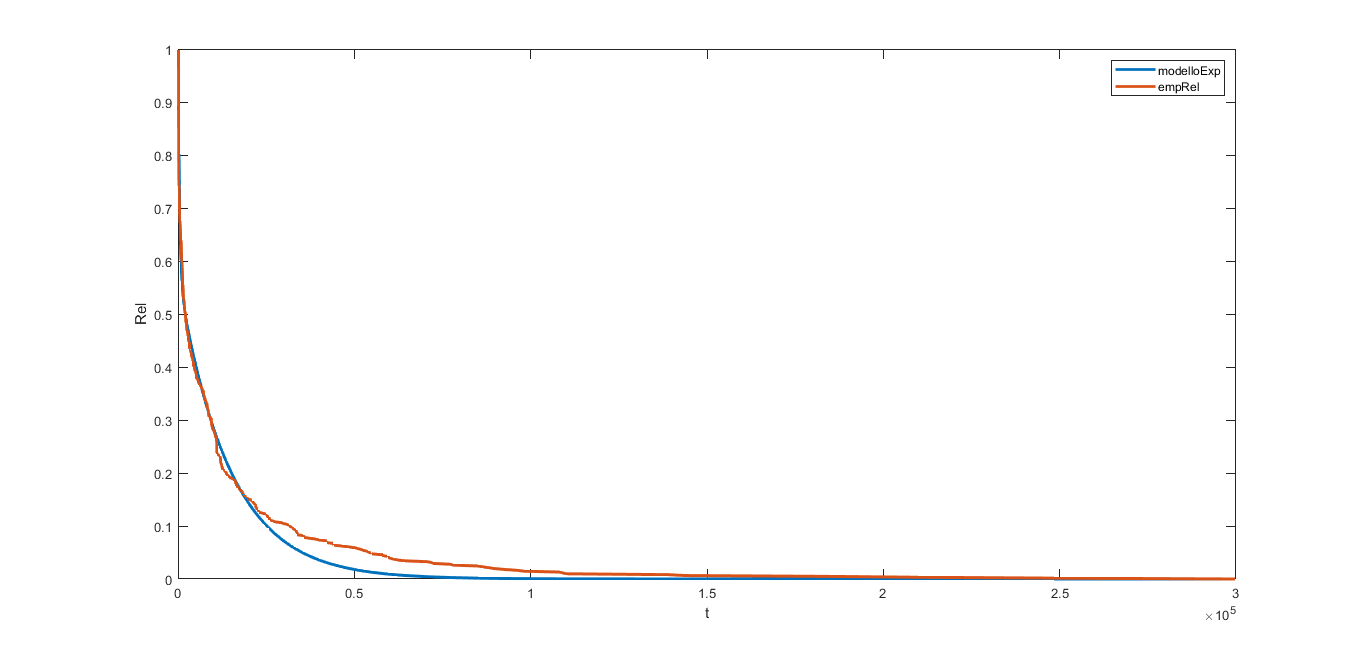
\includegraphics[width=\textwidth]{img/hw6/FittingM.png}
	\caption{\textit{Fitting empRel Mercury con distribuzione Esponenziale}}
\end{figure}
Tale analisi ha prodotto i seguenti risultati:
\begin{equation*}
	\begin{split}
		&SSE = 0,4685\\
		&Rsquare = 0,9872
	\end{split}
\end{equation*}
L' \textit{Rsquare} è un valore abbastanza elevato, a dimostrazione del fatto che la distribuzione esponenziale selezionata spiega gran parte della variazione di quella oggetto del fitting.
\\Come ulteriore dimostrazione della \textit{GOF - Goodness of Fit} è stato eseguito il già precedentemente citato \textit{Kolmogorov-Sminrov test}, il quale ha prodotto come risultato h = 0, verificando l'ipotesi nulla.
\begin{minted}[framesep = 1mm,
	fontsize = \footnotesize,
	breaklines,
	]{MATLAB}
	h = kstest2(empRel,fittedmodel(t));
\end{minted}
\subsubsection{Fitting EmpRel - BlueGene}
Lo stesso procedimento descritto in precedenza è stato iterato per il supercalcolatore Blue-Gene. Anche in questo caso è stata selezionata una distribuzione Esponenziale a 2 termini, come modello che meglio approssima la Reliability empirica del sistema.
\begin{figure}[H]
	\centering
	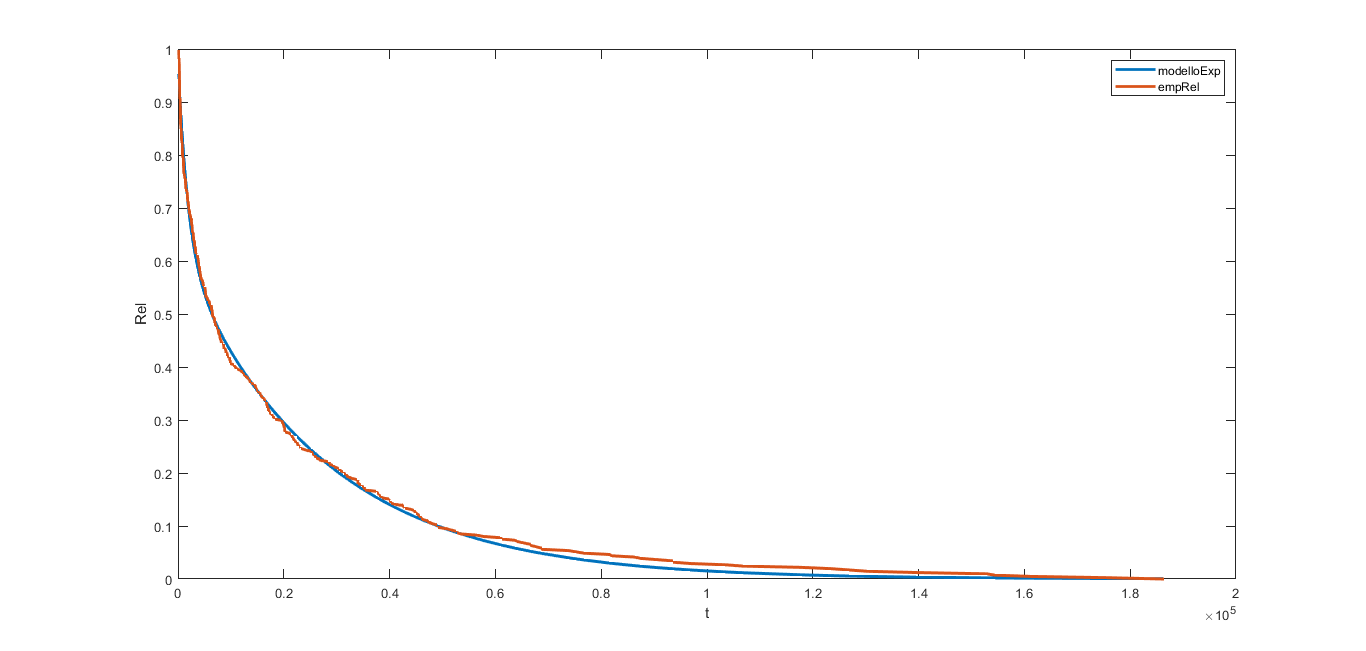
\includegraphics[width=\textwidth]{img/hw6/FittingBG.png}
	\caption{\textit{Fitting empRel Blue-Gene con distribuzione Esponenziale}}
\end{figure}
I risultati prodotti dall'analisi sono i seguenti:
\begin{equation*}
	\begin{split}
		&SSE = 0,08606\\
		&Rsquare = 0,9974
	\end{split}
\end{equation*}
Anche in questo caso il kstest ha fornito output h=0, confermando la bontà del fitting eseguito.
\\
La distribuzione esponenziale è associata a fenomeni degenerativi di tipo hardware (boh vedi meglio ste conclusioni - non sono convita che mercury sia esponenziale SSE non piccolo).
\subsection{Analisi Reliability per Sottocomponenti}
Sono stati eseguiti dei confronti tra Reliability dell'intero sistema e quella relativa ad alcuni dei suoi sottocomponenti, suddivisi per tipologia di nodo. 
\subsubsection{Mercury}
Per ogni categoria di nodo (master, login, computation e storage), sono stati selezionati quelli in cui, in base al report, è stato riscontrato il numero più elevato di fallimenti, effettuando quindi dei confronti "al limite":
\begin{itemize}
	\item \textbf{tg-master},
	\item \textbf{tg-login3},
	\item \textbf{tg-c401},
	\item \textbf{tg-s044}
\end{itemize}
Le entries associate a ciascuno di questi nodi sono state isolate in log specifici, i quali sono stati manipolati con le tecniche già descritte per i log principali. Per tutti i nodi è stata selezionata una finestra temporale di 150. Dopodichè, dagli interarrivi relativi ai singoli nodi sono state calcolate le Reliability Empiriche.
\\
\begin{figure}[H]
	\centering
	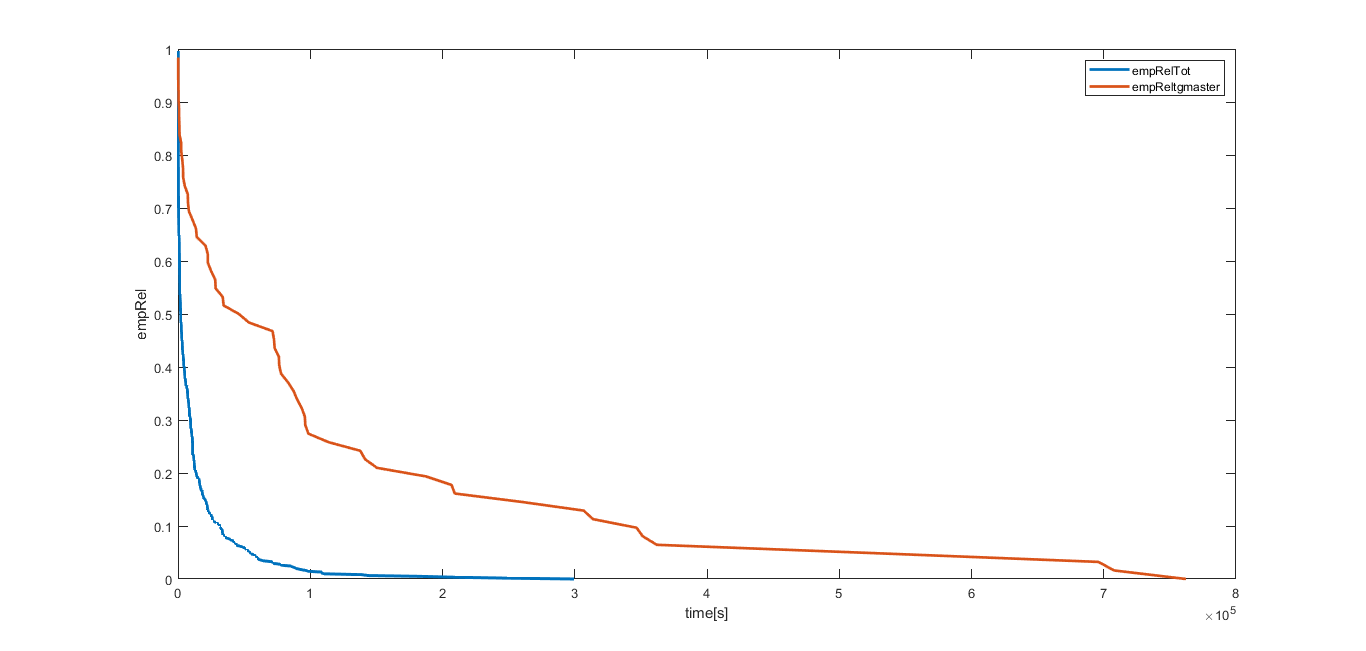
\includegraphics[width=\textwidth]{img/hw6/Rel_Tot_Tgmaster.png}
	\caption{\textit{Confronto Reliability Totale - Reliability tg-master}}
\end{figure}
\begin{figure}[H]
	\centering
	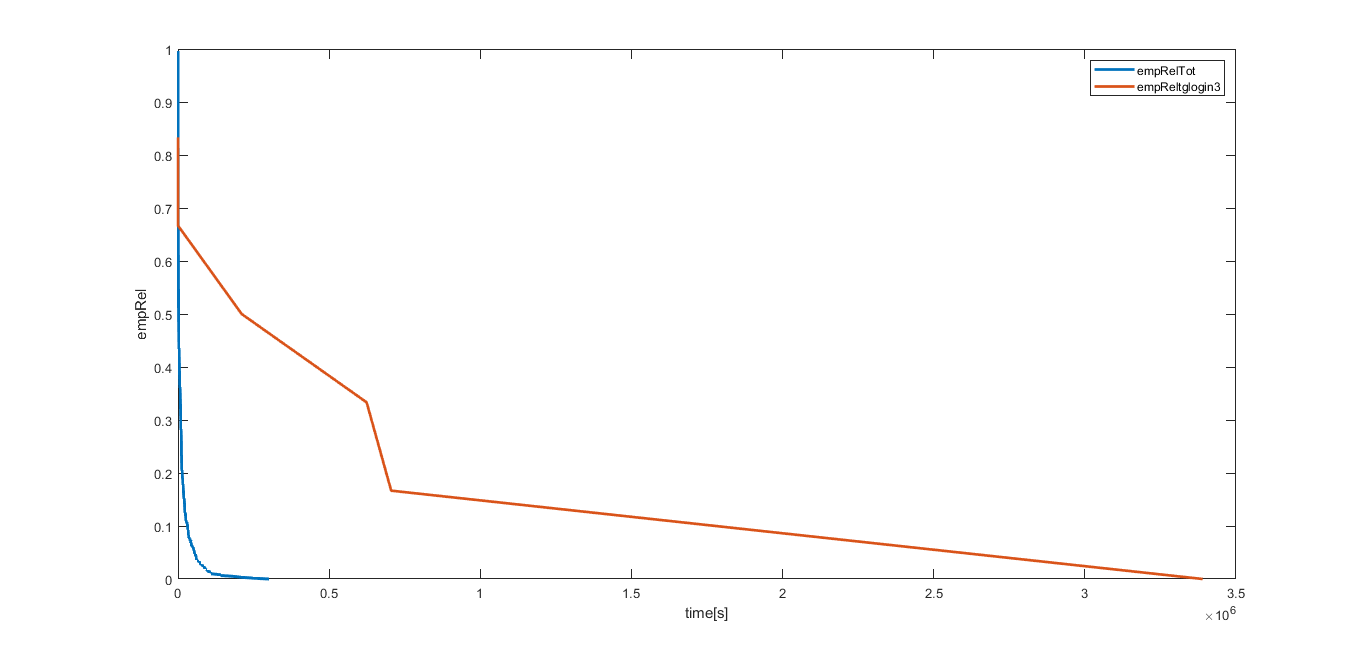
\includegraphics[width=\textwidth]{img/hw6/Rel_Tot_Tglogin.png}
	\caption{\textit{Confronto Reliability Totale - Reliability tg-login3}}
\end{figure}
\begin{figure}[H]
	\centering
	\includegraphics[width=\textwidth]{img/hw6/Rel_Tot_Tgc.png}
	\caption{\textit{Confronto Reliability Totale - Reliability tg-c401}}
\end{figure}
\begin{figure}[H]
	\centering
	\includegraphics[width=\textwidth]{img/hw6/Rel_Tot_Tgs.png}
	\caption{\textit{Confronto Reliability Totale - Reliability tg-s044}}
\end{figure}
Quindi tutti i nodi eccetto il tg-c401, hanno una reliability migliore rispetto a quella totale del sistema. 
\\Il nodo di computation \textbf{tg-c401} per tempi brevi in confronto ai totali, risulta essere il meno reliable, addirittura anche rispetto al sistema. Ciò significa che esso potrebbe essere un probabile collo di bottiglia per il supercalcolatore Mercury. Quest'ultima affermazione è molto probabile in quanto tale nodo è quello caratterizzato dal maggior numero di fallimenti.
\\In seguito è stato riportato un grafico che confronta tra di loro le reliability dei diversi nodi selezionati:
\begin{figure}[H]
	\centering
	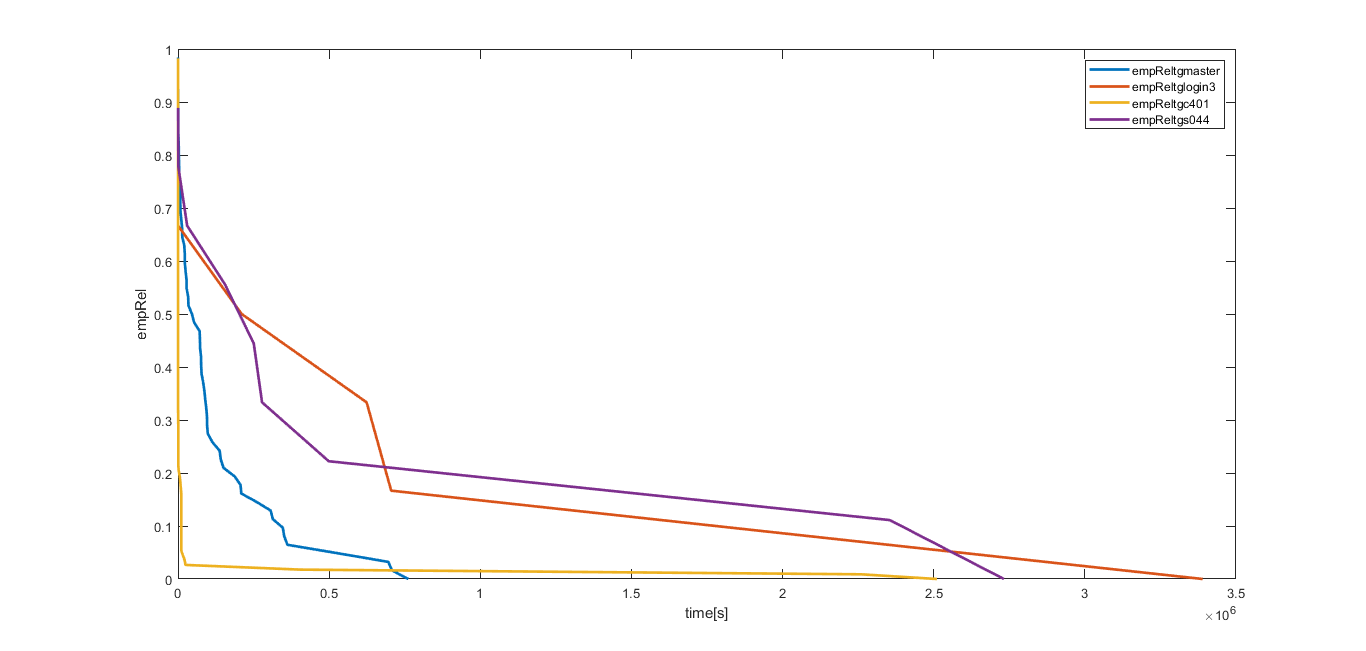
\includegraphics[width=\textwidth]{img/hw6/confrontoMercury.png}
	\caption{\textit{Confronto Reliability Nodi Mercury}}
\end{figure}
Altre considerazioni su quest'ultima immagine pensaci dopo.
\\
\\
Un altro confronto è stato effettuato sulla reliability di nodi funzionalmente simili tra di loro.
\\Per tale analisi sono stati selezionati tre nodi computation:
\begin{itemize}
	\item \textbf{tg-c401}, il nodo con il numero maggiore di fallimenti,
	\item \textbf{tg-c238},
	\item \textbf{tg-c242}.
\end{itemize}
Gli ultimi due presentano un numero di fallimenti molto simile tra di loro.
\begin{figure}[H]
	\centering
	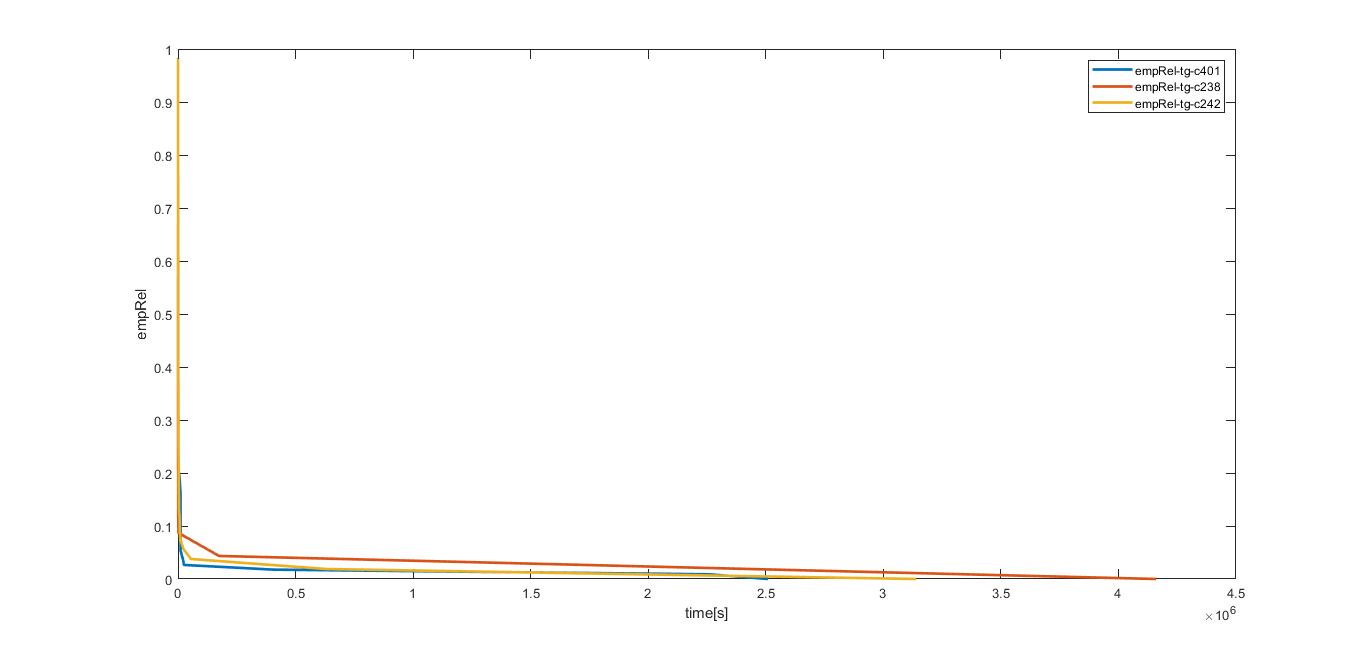
\includegraphics[width=\textwidth]{img/hw6/RelCompMercury.png}
	\caption{\textit{Confronto Reliability Nodi Computation Mercury}}
\end{figure}
La reliability del nodo 401 risulta essere sempre peggiore delle altre, anche se nonostante ciò gli andamenti risultano essere tutti molto simili tra di loro (rispettivamente 1273 e 1067). Tutti i nodi computation analizzati hanno dunque una reliability molto bassa.
\subsubsection{Blue-Gene}
L'analisi è stata ripetuta anche per i primi 3 nodi con più entries di fallimenti di Blue-Gene. Essi, ordinati per numero di entries, sono:
\begin{itemize}
	\item \textbf{R71-M0-N4},
	\item \textbf{R12-M0-N0},
	\item \textbf{R63-M0-N2}
\end{itemize} 
\begin{figure}[H]
	\centering
	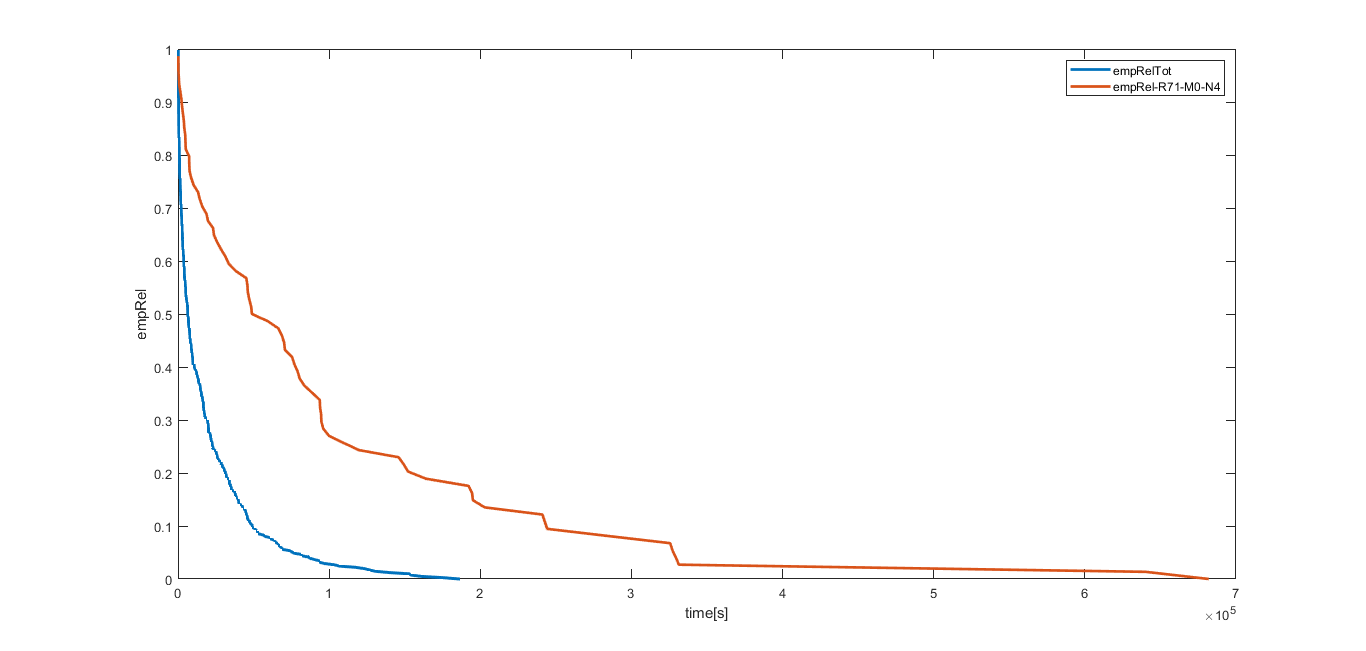
\includegraphics[width=\textwidth]{img/hw6/Rel_Tot_R71.png}
	\caption{\textit{Confronto Reliability Totale - Reliability R71-M0-N4}}
\end{figure}
\begin{figure}[H]
	\centering
	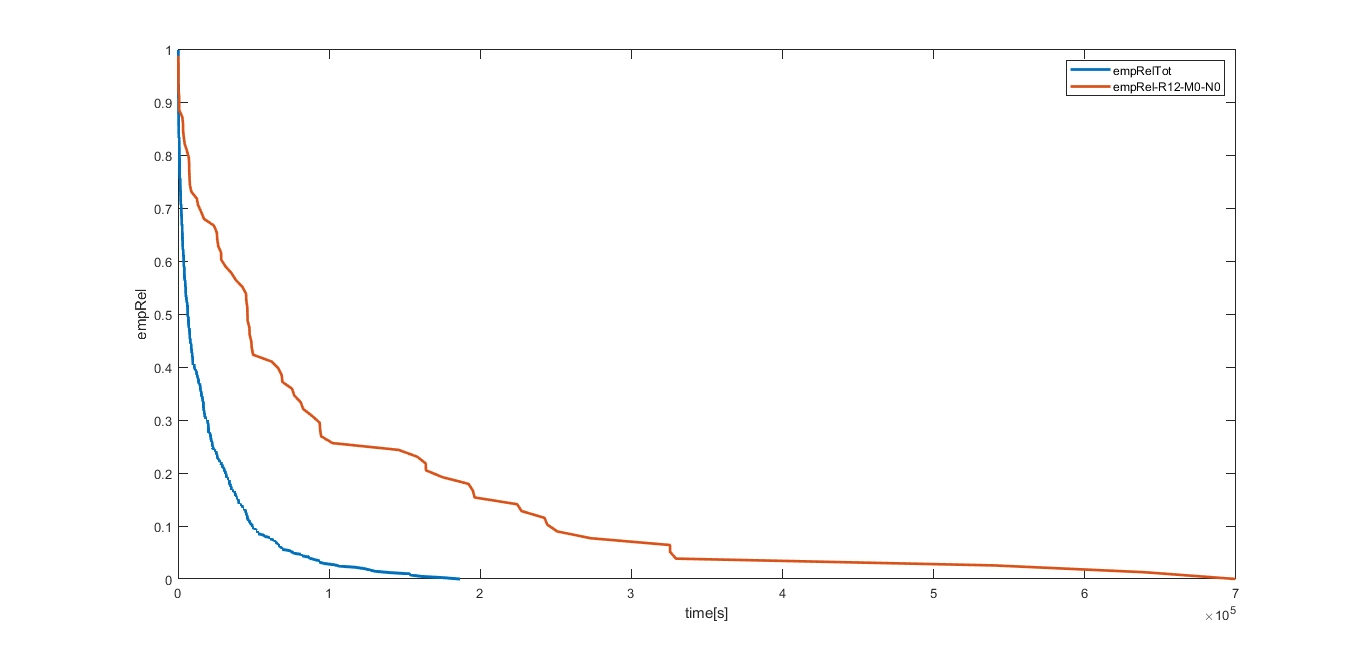
\includegraphics[width=\textwidth]{img/hw6/Rel_Tot_R12.png}
	\caption{\textit{Confronto Reliability Totale - Reliability R12-M0-N0}}
\end{figure}
\begin{figure}[H]
	\centering
	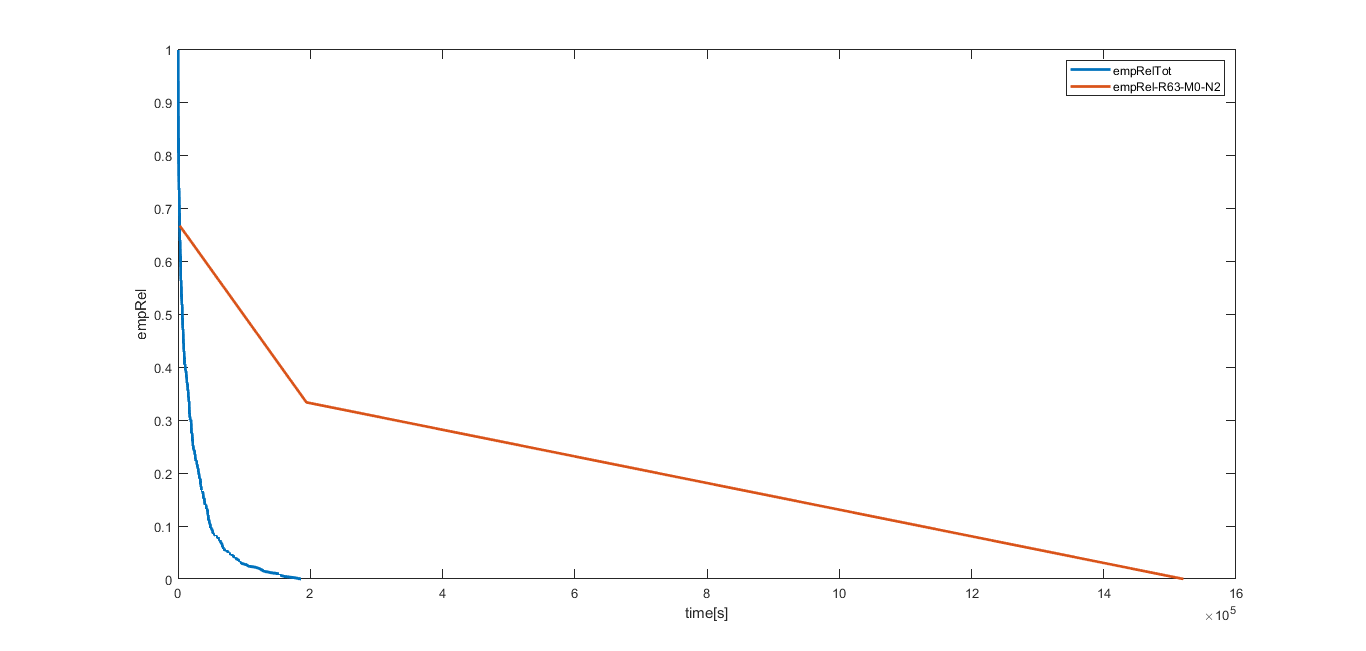
\includegraphics[width=\textwidth]{img/hw6/Rel_Tot_R63.png}
	\caption{\textit{Confronto Reliability Totale - Reliability R63-M0-N2}}
\end{figure}
In tal caso non risultano esserci evidenti colli di bottiglia, e la reliability del singolo nodo risulta essere sempre maggiore di quella totale del sistema.
\\Anche per Blue-Gene si riporta un grafico in cui vengono messe a confronto le reliability dei 3 differenti nodi:
\begin{figure}[H]
	\centering
	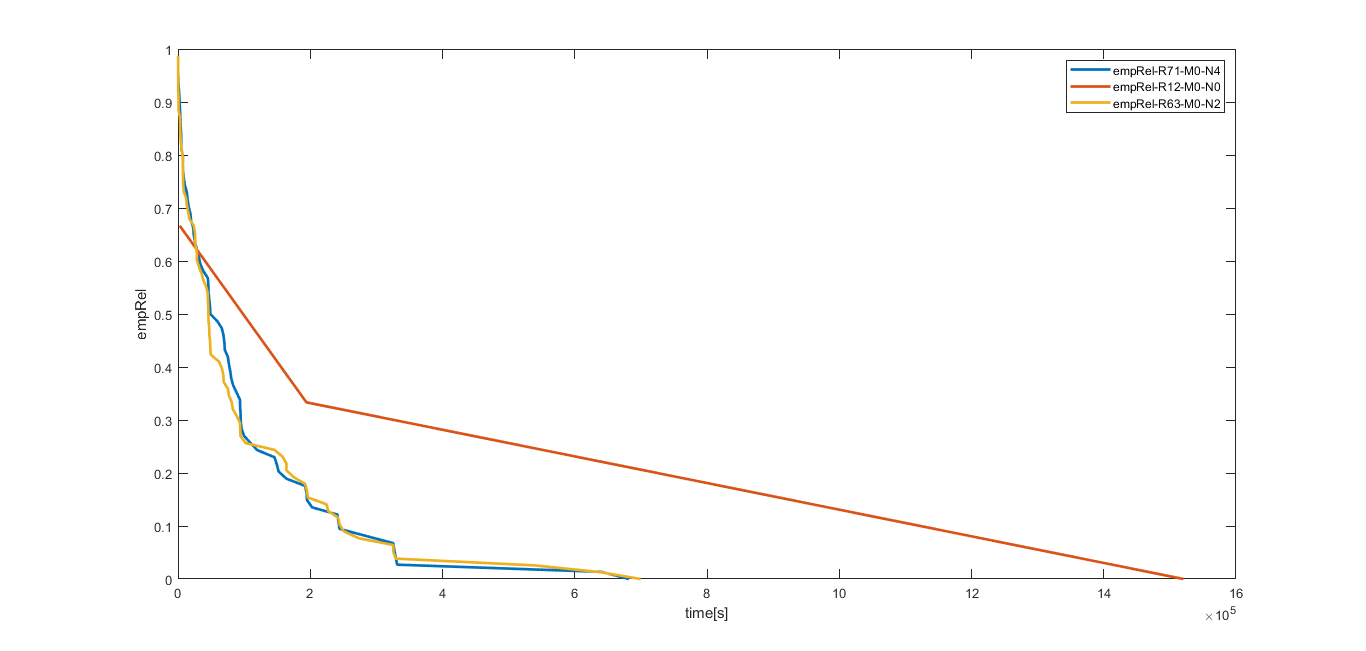
\includegraphics[width=\textwidth]{img/hw6/confrontoBG.png}
	\caption{\textit{Confronto Reliability Nodi Blue-Gene}}
\end{figure}
In tal caso i nodi confrontati sono tutti funzionalmente simili. Come si evince dal grafico la reliability del nodo \textbf{R71-M0-N4} e \textbf{R63-M0-N2} risulta avere un andamento molto simile, a differenza del terzo nodo il quale è più reliable dei precedenti.
\subsection{Domanda 5}
Esiste una relazione tra tipo di errore e nodo(mercury)?

